\documentclass[preprint,12pt]{article}

\usepackage{algorithmic}
\usepackage{algorithm}
\usepackage{enumerate}
\usepackage{enumitem}
\usepackage{graphics}
\usepackage{graphicx}
\usepackage{geometry}
\usepackage{amsmath}
\usepackage{wrapfig}
\usepackage{subfig}
\usepackage{framed}
\usepackage{color}
\usepackage{soul}
\usepackage{bm}

\usepackage{multirow}
\usepackage[T1]{fontenc}
\usepackage[latin9]{inputenc}
%\usepackage{units}
\usepackage{esint}

\geometry{legalpaper,  margin=1in}

\newcommand{\CM}[2][green]{ {\sethlcolor{#1} \hl{#2}} }
\newcommand{\KB}[2][cyan]{ {\sethlcolor{#1} \hl{#2}} }

%\makeatother

%\usepackage{babel}fs

\begin{document}
\title{An Empirical Bayesian Framework for Assessing Partisan Bias in Redistricting Plans}

\author{Kevin Baas and Colin McAuliffe}

\maketitle

\begin{abstract}
We present a framework for assessing partisan bias in redistricting plans using an empirical Bayesian approach, as well as a new metric for measuring partisan bias called the specific asymmetry.
Given at least one observation of the election results in a state, we estimate a probability model representing likely future election outcomes.
The expected value of the specific asymmetry is then computed by sampling from the model using the Monte Carlo method.
Redistricting plans which have an expected asymmetry of zero may be considered fair, since on average neither of the two major parties will be given an advantage.
Conversely, redistricting plans which have a nonzero expected asymmetry may be considered to be unfair, since partisan bias is a persistent feature of the plan.
This analysis technique is applied to the United States congressional elections from 1972-2016 to examine the total and net effects of partisan bias in recent history.
We also examine the post 2010 census Wisconsin State Assembly, which is the subject of \emph{Whitford v. Gil}.

\end{abstract}

\section{Introduction}
In the United States, the process of drawing districts for a state's legislative bodies and federal congressional delegation is usually in the hands of that state's legislature.
Partisan state legislatures have used the redistricting process in pursuit of various goals such as incumbent protection, maximizing their share of seats, and even diluting the voting power of citizens on the basis of race.
Opportunities to manipulate the redistricting process for partisan advantage abound, particularly with the advent of sophisticated algorithms for redistricting as well as a high degree of partisan and geographic polarization in the current political climate.
However, the supreme court has yet to rule definitively on the justicability of partisan gerrymandering, and recent rulings suggest that a manageable standard for measuring gerrymandering is a prerequisite for a ruling on justicability CITE.

A ruling on the justicability of partisan gerrymandering would have significant consequences for democracy in the United States.
Partisan gerrymandering not only distorts the composition of legislative bodies, it represents a dilution of the voter's ability to attempt to influence policy by electing representatives of their choosing.
The ability of state legislatures to use redistricting to influence the outcome of elections comes at the direct expense of voter's ability to use their ballot to influence the outcome of elections.
However, in order to properly asses the harm caused by partisan gerrymandering, courts require mathematical tools for analyzing partisan bias in a redistricting plan.

Development of a standard that fits with existing rulings, accurately measures partisan bias under generic conditions, and is simple enough to be effectively communicated to a court is not an easy task.
For example, a common sense standard might be to require that a party's share of seats is proportional to its share of votes, which is simple and applicable to swing states as well as more partisan states.
However, even when redistricting is fair, single winner voting systems tend not to produce such proportional outcomes CITE, and the supreme court has stated that proportionality is not acceptable CITE.
A second example is the mean median difference test CITE, which fits with existing rulings since it measures partisan bias without regard to proportionality and is simple enough to be calculated by a judge without an expert witness.
However, it is only effective in measuring bias for states which are close to even in terms of partisanship CITE: 
\KB{I'M NOT SURE THERE'S A CITATION FOR THIS - IT MIGHT BE A NOVEL STATEMENT.}
\CM{I believe it is discussed specifically for mean-median by Sam Wang in his ELJ article, will double check}

Several standards have been proposed in literature, and for clarity we describe a standard as consisting of two parts.
The first part is a metric, which is some quantity that can be calculated from a given election result and is a measure of the unfairness or bias.
The second part is a model (or in the absence of a statistical model per se an analysis of the metric in historical elections), which allows one to asses whether or not the observed value of the metric can be regarded as the result of chance in an otherwise unbiased redistricting plan, or if bias is a persistent feature of the plan.
For example, the plaintiffs in Whitford v. Gil used a metric called the efficiency gap CITE, which measures the discrepancy in the so called wasted votes between the two major parties.
An examination of historical election data determined that it is reasonable to assume that observing an efficiency gap of greater than 7\%.
Grofman and King proposed a metric based on the deficit in seats at 50\% votes in a seats votes curve CITE, and Nagle has proposed several other metrics based on the seats votes curve, including the geometric area between the seats votes curve and its reflection.

A special group of standards are those where a particular metric is associated with an existing analytic statistical model.
Among these are the lopsided wins test, the mean median difference test, and the chi square test proposed by Wang CITE.
These standards are attractive because they are based on statistics with properties that are well understood, that are used broadly for applications across many fields, and are relatively simple.
However, these tests have some drawbacks.
Namely, the models used for computing the significance level for those tests are valid asymptotically as the number of districts increases, meaning that the statistical power of these standards is diminished for states with just a few districts.
Additionally, these models assume that samples are independent and identically distributed (IID), which is an assumption that is crucial for the tests to be analytic (and hence simple) but not necessarily realistic for elections.
For instance, the IID assumption would imply that the probability of a deeply partisan Republican district being won by a Republican is the same as the probability of a deeply partisan Democratic district in the same state being won by a Republican.
The effects of small sample sizes are discussed in the statistics literature CITE, and the effect of the IID assumption is an area we are currently investigating.

Another group of standards are those based on Monte Carlo simulation CITE.
The main advantages of Monte Carlo based standards are flexibility, since they can be used with a wide variety of metrics or even multiple metrics in combinations, and robustness.
An example is test III proposed by Wang CITE, where the metric used was the proportion of seats won by a party, and the model was a Monte Carlo technique where 'fantasy' congressional delegations were sampled from national congressional voting results.
This method can be used to establish whether or not a party's vote share wins them seats excessively relative to a national baseline.
The standard that we propose is also based on Monte Carlo simulation.
The metric, which we refer to as the specific asymmetry (see section \ref{sec:MB}), is a measure of partisan bias that determines discrepancy in seats won by the losing party under a reversal in statewide partisanship.  
The model, described in section \ref{sec:FB}, uses a Monte Carlo technique based simulations of an empirically estimated probability model for district and statewide partisanship.
The drawback of Monte Carlo based standards is complexity.
In fact, despite the fact that Monte Carlo simulation is a common and highly conventional technique, the supreme court has expressed skepticism of this type of approach CITE \KB{I'M NOT SURE THAT'S TRUE}\CM{you may be right, I have a vague reccolection on this but I'll need to look further}.
Whether or not a court can be convinced to warm up to such an approach has yet to be determined, but what is clear is that Monte Carlo based methods are powerful tools for examination of bias and robustness.

The empirical Bayesian framework that we propose is not only appropriate for assessing bias that has existed in past redistricting plans, but it is useful for understanding how bias could be introduced into future redistricting plans, even as strategies for gerrymandering change in response to the introduction of a hypothetical standard.
In fact, the empirical Bayesian model that we propose is compatible with all of the metrics we have discussed thus far, and can be used as part of a standard itself, or can be used to test the robustness of standards that do not require Monte Carlo simulation. 
We therefore contend that regardless of whether or not the approach we present is an acceptable judicial standard itself, it remains a powerful tool for assessing partisan bias in redistricting plans that will prove useful for researchers and advocates of redistricting reform.
For example, the Monte Carlo technique can be used to evaluate the properties of metrics which do not have well known analytic statistical properties such as the efficiency gap and the specific asymmetry metric proposed in section \ref{sec:MB}, or to evaluate the effect of the IID assumption for metrics which do have known analytic properties such as the mean median difference and the t-test.
Additionally, the technique could be used to help develop an understanding of the conditions where different metrics may agree or disagree with one another.
For fast reference, table \ref{tab:Stand} summarizes each of the standards discussed here. 

\begin{table}[htb!]
\centering
\caption{Summary of the metrics and models employed by various gerrymandering standards \label{tab:Stand}}
\begin{tabular}{|l|l|l|}
\hline
Standard & Metric & Model\\
\hline
\hline
Grofman and King & Deficit in Seats at 50\% of the vote & ?\\
\hline
Mean Median Difference & mean median difference & asymptotic distribution \\
 &                                              & assuming IID samples CITE\\
\hline
Chi square test & mean median difference & asymptotic distribution \\
                &                        & assuming IID samples CITE\\
\hline
Lopsided wins test & difference in party  & asymptotic distribution \\
                   &  mean winning vote share & assuming IID samples CITE\\
\hline
Test III & Party seat share & MC sampling of national \\
         &                  & district voting results\\
\hline
Chen and Rodden & Party seat share & MC sampling of randomly \\
         &                         & generated districting plans\\
\hline
Present study & Specific Asymmetry & MC sampling of the \\
              &                    & empirical Bayesian model\\
\hline
\end{tabular}
\end{table}

\section{Measuring Bias with the Specific Asymmetry\label{sec:MB}}

Measuring partisan bias accurately presents several challenges from a mathematical and legal perspective.
Redistricting will always be an artificial process, and therefore we must establish what characteristics of a redistricting plan can be regarded as normative before attempting to measure deviations from the normative standard.
We propose the following definition: \emph{a fair redistricting plan is one that, on average, will not be biased in favor of either of the two major parties}
With this definition in mind, we turn our attention to several challenges in devising a metric for bias.
First, single winner elections tend not to produce proportional outcomes CITE, and we therefore can not use proportionality or the lack thereof as a measure of bias.
Bias should therefore be a measure of symmetry, which permits disproportionate outcomes but requires that any advantage that might arise from the disproportionate nature of the single winner election system be equally available to either party.
In other words, we say that the result is unbiased if and only if any advantage gained by a party, above what is proportional, is a consequence of the disproportionate nature of the single winner election system, and not an additional advantage piled on top of that.

A few measures of bias that follow this definition exist in the literature, such a Grofman and King, and the mean median difference CITE.
However, these measures of bias tend to apply only to states which are close to 50-50 partisanship CITE.
For more partisan states, these measures become more difficult to interpret except as the bias which could have occurred had the partisanship in the state in question been closer to even.
Another approach is to consider the bias at levels of partisanship by using the geometric area between the seats votes curve and its reflection CITE.
Useful information may be gleaned from these approaches, but Justice Kennedy expressed a dislike for measures based on a hypothetical state of affairs.
Additionally, measurement of bias at different levels of hypothetical partisanship may lead to significantly different results depending on the partisanship level considered.
For example, the seats votes curve for the Wisconsin state assembly shows substantial bias favoring Republicans at close to even partisanship, but the complete reverse at high levels of Democratic partisanship.
This means that bias measures which do not consider the actual partisanship in a state could result in false positives and false negatives.
In light of this, a measure of bias that is applicable to any level of partisanship and that directly considers the actual level of partisanship in a given state seems appropriate.
To address these challenges, we propose a measure of bias which we call the specific asymmetry, which is the deviation of the seats votes curve from the symmetry line measured at the statewide popular vote.

Bias by any measure may occur by chance in an otherwise fair redistricting plan, it is even possible for an antimajoritarian outcome to result from chance.
It is also important not only to consider the harm a plan has caused to voters, but to also seek to assess the likelihood that a plan will cause harm to voters in future elections.
For example, the plaintiffs in \emph{Whitford v. Gil} argued that based on an examination of a large body of election data, an observed efficiency gap of greater than 7\% in a given election was strongly suggestive that bias in favor of the redistricting party would persist.
In other words, the observation of a large bias was not only indicative of harm to voters that had already occurred, but it was also a strong predictor of likely future harm to voters.
Analysis of historical data is not the only way to assess likely future harm due to bias, and we would like to use a method that takes advantage of as much specific information about the redistricting plan in question as possible.
Therefore we employ an empirical statistical model to determine whether a particular redistricting plan will be unbiased \emph{on average}, or if bias is a persistent feature of the plan.
This allows us to distinguish between chance occurrences of bias on an otherwise fair map, and to asses the magnitude of likely future harm a map can be expected to cause. 
Full details of the particular model employed here are presented in the following section.


\section{Modeling the Likelihood of Bias in Future Elections\label{sec:FB}}

\section{Partisan Bias in the U.S. Congress 1972-2016\label{sec:Hist}}
We present an examination of partisan bias in the United States congress for elections from 1972 to 2016 by computing the expected specific asymmetry for each state and redistricting cycle using 10,000 Monte Carlo samples, as well as the observed specific asymmetry for each state and election.
First, we consider the net asymmetry, which is indicative of how gerrymandering may have affected the partisan composition of congress.
In figure \ref{fig:NetAsym}, the net observed asymmetry is shown for each election.
The expected net asymmetry for each redistricting cycle is also shown with 50\% and 90\% confidence intervals.
A progression is observed where the net asymmetry strongly favored Democrats in the 70's and 80's, mildly favored Democrats in the 90's, was roughly zero net asymmetry in the 2000's, and strongly favored Republicans in the 2010 cycle.
Histograms for the simulations can be found in figure \ref{fig:NetAsymHist}, which shows the expectation and variance of the net specific asymmetry.
In the 80's for example, Democrats could expect about 20 seats on average due to redistricting bias, with a negligibly small probability that the net national asymmetry would favor Republicans.
This situation has reversed entirely by the 2010 cycle, where Republicans can expect 18 seats on average due to redistricting bias.
Interestingly the 2000's show zero net bias on average, but this does not mean that the country was free of gerrymandering.
As we will show later in this section, there was significant gerrymandering by Republicans and Democrats in their respective territories, but the net effect of these gerrymanders tended to roughly cancel.
\begin{figure}[htb!]
    \begin{center}
        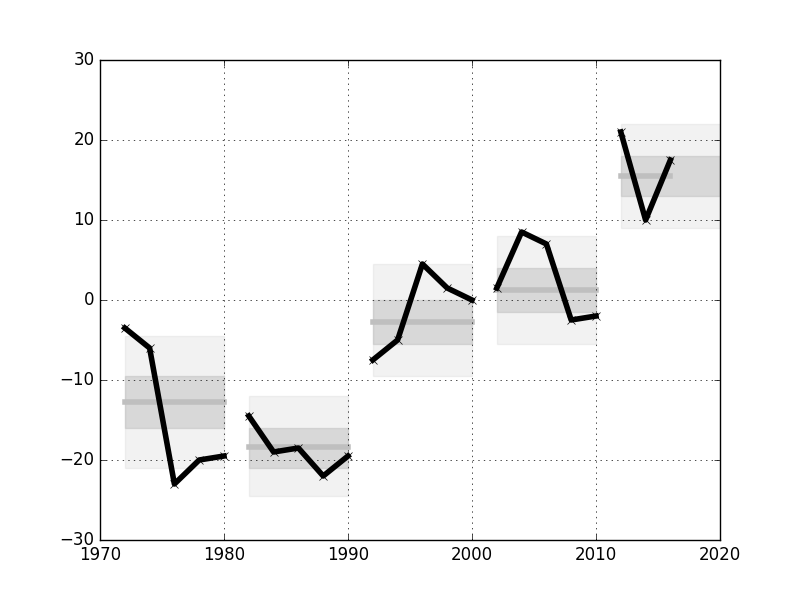
\includegraphics[scale=0.6]{../Figures/ExpectedAsymmetry/netAsym.png}
        \caption{Net national asymmetry based on 10,000 simulations}\label{fig:NetAsym}
    \end{center}
\end{figure}
\begin{figure}[htb!]
    \begin{center}
        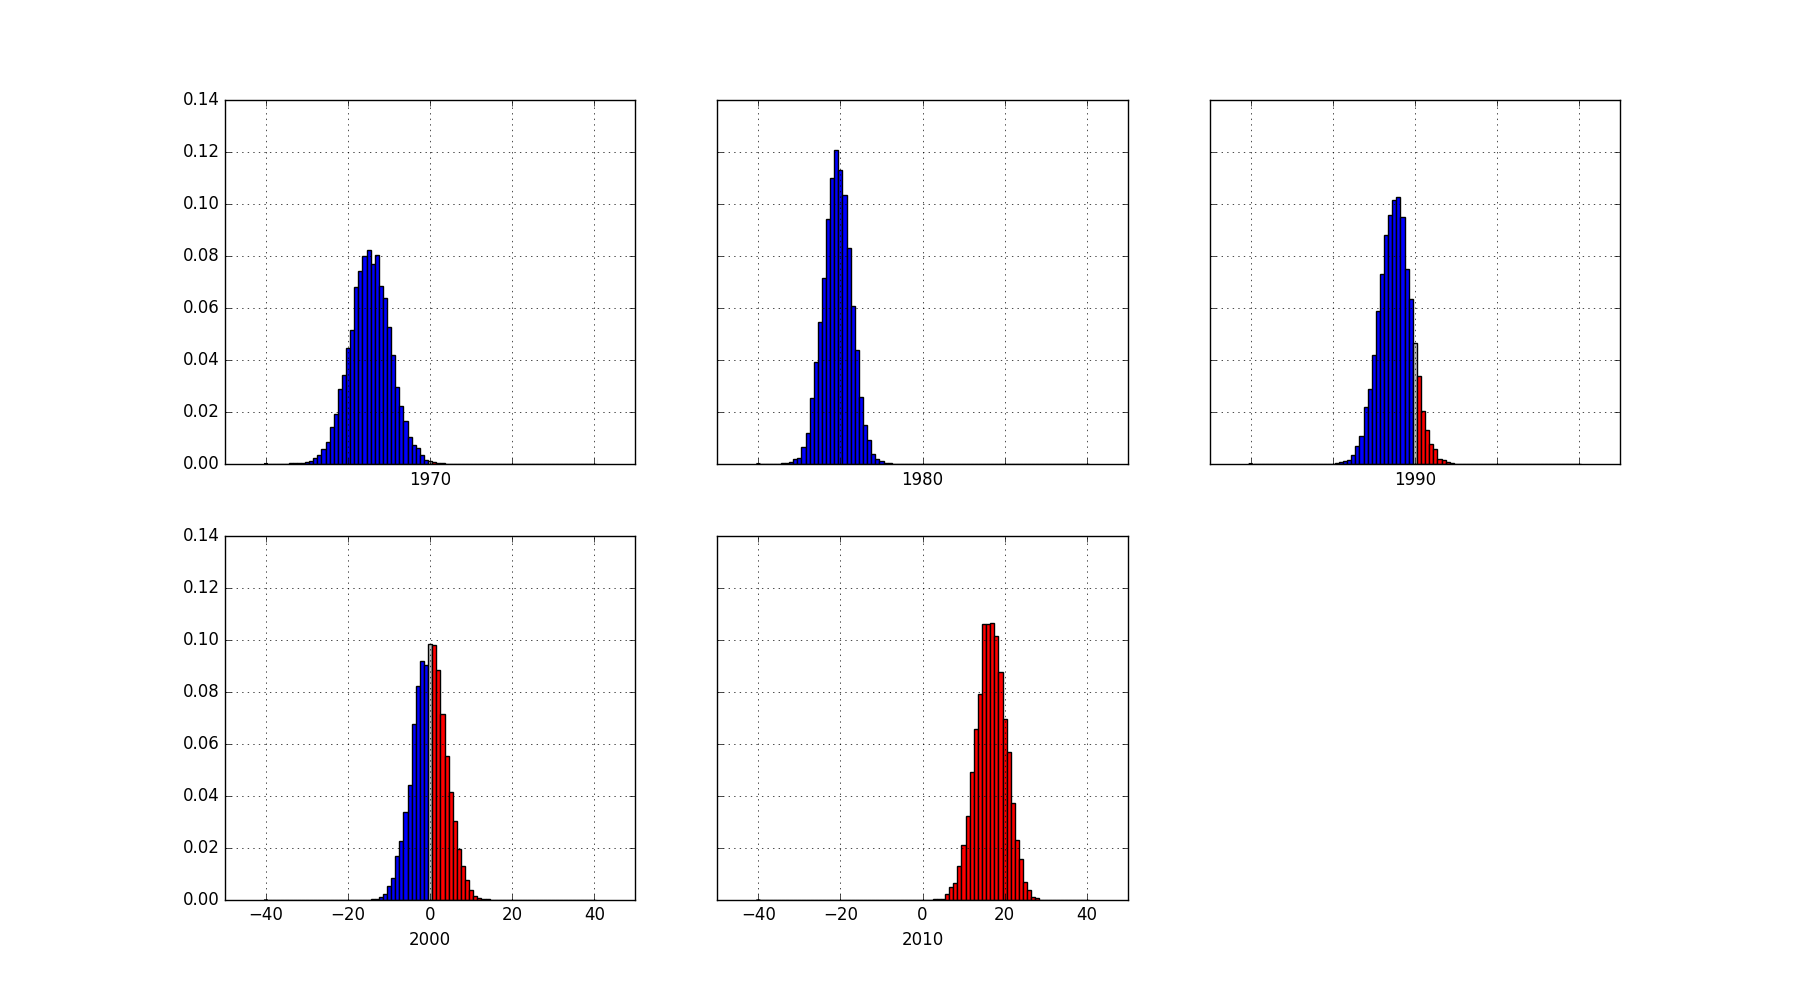
\includegraphics[scale=0.4]{../Figures/ExpectedAsymmetry/netAsymHist.png}
        \caption{Net national asymmetry based on 10,000 simulations}\label{fig:NetAsymHist}
    \end{center}
\end{figure}

The results for the 2010s showing significant Republican gerrymandering are consistent with the well known REDMAP program, where Republicans lead a highly successful effort to gain control of several state houses in advance of the 2010 redistricting.
For earlier cycles, we observe qualitative agreement with similar studies CITE in terms of which party benefited on net from gerrymandering.
Quantitatively, we observe some disagreement in terms of the magnitude of gerrymandering, with the present approach attributing more seats to redistricting bias.
This can be explained by differences in the analysis methodology.
The simulation technique employed in CITE draws a 'fantasy' delegation from national voting results in order to determine if a party is winning seats excessively relative to its vote share.
National voting results are used as a baseline, but this baseline itself may contain substantial bias, which means only large gerrymanders will be successfully identified. 
In contrast, the present approach does not use a national baseline, and instead detects asymmetry in each state on a case by case basis.

Differences in methodology aside, the result that the expected asymmetry favoring Democrats in the 80's is larger than that favoring Republicans in the 2010 cycle is surprising.
In the 2010 cycle, Republicans had the advantages of sophisticated redistricting algorithms, a high degree of geographic polarization, and low variability in voter preferences.
These factors enable effective gerrymandering and would not have been available to redistricters in the 80's.
On the other hand, Democrats controlled a significant number of states in the 80's and the national level of Democratic partisanship in congressional elections was fairly high, while it is closer to even in the 2010 cycle.
Compared to Republicans in the 2010 cycle, Democrats in the 80's obtained seats due to small levels of bias in a number of states, and additionally obtained significant numbers of seats in larger states like California and Texas.
Figure \ref{fig:80vs10} compares the simulated asymmetry distributions for California and Texas in the 80's and for Pennsylvania and North Carolina in the 2010's.
We can see that the variability of the asymmetry in Texas and California was higher than that of Pennsylvania and North Carolina.
It is also worth noting that the number of seats available in these states in the cycles under consideration.
In the 80's Texas has 24 seats and  California had 43, while in the in the 2010's, Pennsylvania had 18 seats and North Carolina had 13.
More district lines offers more opportunities for parties to manipulate redistricting to obtain a partisan advantage, and as a fraction of available seats, the gerrymanders in Pennsylvania and North Carolina are truly remarkable.
This is consistent with the fact that conditions and technology to produce highly stable gerrymanders would exist to a greater degree in the 2010s than in the 1980s.

\begin{figure}[htb!]
    \begin{center}
        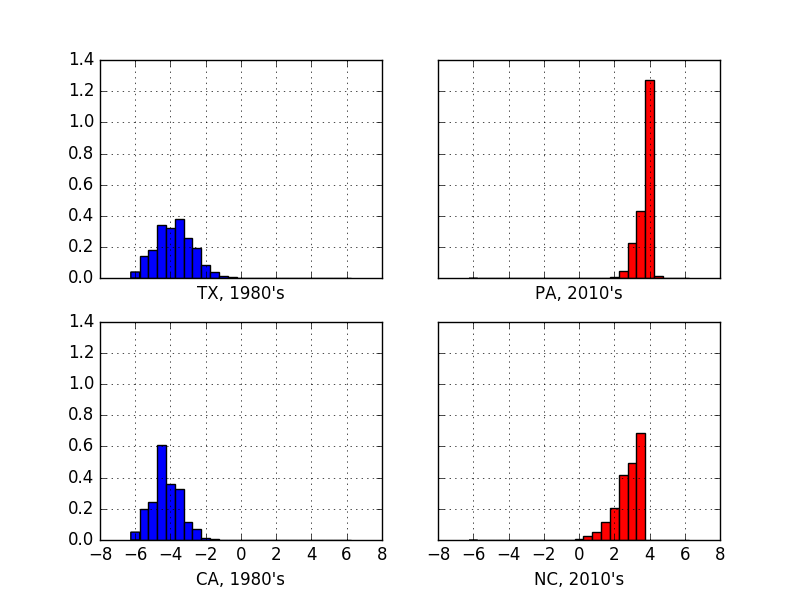
\includegraphics[scale=0.4]{../Figures/ExpectedAsymmetry/80vs10.png}
        \caption{Histograms of the simulated asymmetries in Texas and California in the 1980's, and Pennsylvania and North Carolina in the 2010s}\label{fig:80vs10}
    \end{center}
\end{figure}

Net zero gerrymandering is preferable to a distorted congress, but net zero gerrymandering may still result in the congressional delegations of individual states being highly distorted.
We would therefore also like to examine the total asymmetry, or the sum of asymmetries in all states without regard to which party the asymmetry favors.
This tells us to what extent redistricting is being used to control election outcomes nationally.
This is plotted for each election cycle in \ref{fig:totalAsym}, where we observe that the total asymmetry has held fairly constant over each cycle.
\KB{GOOD PLACE TO MENTION THAT ELECTIONS ARE A ZERO-SUM GAME - THAT TO THE EXTENT THAT THE REDISTRICTERS DETERMINED THE OUTCOME - THE VOTERS DID NOT.}
\CM{agree will add}
Since there is a fixed number of seats available, every seat of partisan bias that redistrictors secure by gerrymandering is an equal amount of representation taken away from voters.
In other words, the relationship between voter representation and partisan bias resulting from redistricting is that of a zero-sum game: what one side gains, the other side loses.
Regardless of which party benefited from bias on balance, bias in redistricting appears to have affected the representation of millions of voters, for every congressional election since 1972.
\begin{figure}[htb!]
    \begin{center}
        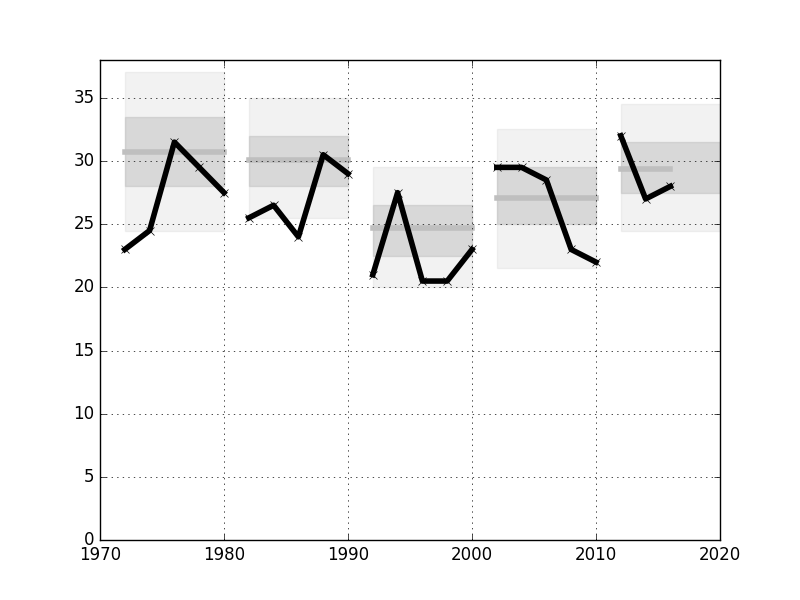
\includegraphics[scale=0.6]{../Figures/ExpectedAsymmetry/totalAsym.png}
        \caption{Total national asymmetry based on 10,000 simulations}\label{fig:totalAsym}
    \end{center}
\end{figure}

While the total national asymmetry has held roughly constant over time, that is not to say that gerrymandering practices have held constant.
To the contrary, some aspects of the 2010 redistricting cycle are quite unprecedented.
Simultaneously, asymmetry has reduced in some states (at least in part due to redistricting reforms enacted in some of those states), while asymmetry has exploded in others.
States known to have been targeted by the REDMAP program are gerrymandered very aggressively in terms of the number of seats available and the level of partisanship in those states.
We can visualize how extreme the most aggressive gerrymanders are in each cycle are by sorting the expected asymmetry (as a percentage of available seats) in descending order for each state.
States with fewer than five seats are excluded since small asymmetries result as very large percentages.
This is shown in figure \ref{fig:asymRank}, where the 2010 cycle stands out as having three states with expected asymmetries that exceeded anything seen previously: Pennsylvania (19.7\%), North Carolina (19.5\%), and Georgia (16.7\%)
Following these are Virginia (13.3\%), Michigan (12.4\%), Ohio (11.6\%), and Wisconsin (10.8\%), which each have large asymmetries by historical standards.
All of these states showed a sudden increase in asymmetry in favor of Republicans after the 2010 redistricting, see table \ref{tab:Asym2000to2010}. 
\KB{PROOF?  CHART?}
\CM{Added a table. I can add more states to the table if that is of interest as well, it's all generated by the script.}
In contrast, California and New York had substantial asymmetries favoring Democrats in the 2000 cycle, and while they still show asymmetries favoring Democrats in the 2010 cycle, the magnitude of the asymmetry has decreased.
\CM{I believe CA implemented an independent commission starting in 2010}
Previous cycles may have had moderate asymmetries in a larger number of states, but in terms of extreme gerrymandering, there has been no time since the Supreme Court ruled in \emph{Reynold v. Sims} (1964) that congressional districts must have roughly equal population, that is comparable to the 2010 cycle.

\begin{figure}[htb!]
    \begin{center}
        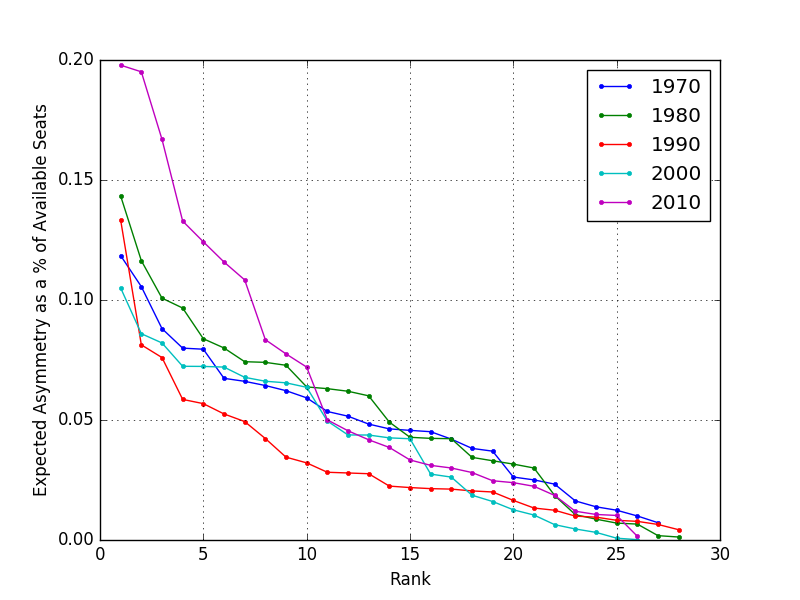
\includegraphics[scale=0.6]{../Figures/ExpectedAsymmetry/asymRank.png}
        \caption{Expected asymmetry as a percentage of seats ranked in descending order for each redistricting cycle}\label{fig:asymRank}
    \end{center}
\end{figure}

\begin{table}[htb!]
\centering
\caption{Change in Expected Specific Asymmetry from 2000 to 2010 for states with large asymmetries in 2010 \label{tab:Asym2000to2010}}
\begin{tabular}{|l|l|l|l|}
\hline
State & Expected Specific     & Expected Specific & Net Change\\
      & Asymmetry, 2000 Cycle & Asymmetry, 2010 Cycle & \\
\hline
\hline
Pennsylvania & R 6.48\% & R 18.70\% & R 12.22\\
\hline
North Carolina & D 4.56\% & R 17.94\% & R 22.51\\
\hline
Georgia & R 3.74\% & R 16.22\% & R 12.48\\
\hline
Virginia & R 6.86\% & R 12.06\% & R 5.20\\
\hline
Michigan & R 6.53\% & R 11.63\% & R 5.10\\
\hline
Ohio & R 7.72\% & R 10.82\% & R 3.10\\
\hline
Wisconsin & D 2.01\% & R 9.90\% & R 11.91\\
\hline
California & D 8.48\% & D 2.17\% & R 6.31\\
\hline
New York & D 7.52\% & D 3.49\% & R 4.04\\
\hline
Illinois & R 0.83\% & D 2.96\% & D 3.79\\
\hline
\end{tabular}
\end{table}


\KB{rough sketch of adding in results about popular vote and removing asymmetry follows}

In figure (x), we compared the actual percentage of congressional seats won by Republicans, with what it would be with the specific partisan asymmetry removed, and then in turn, both of those with the percentage of the popular vote won by Republicans.
 
The results show that, despite the natural multiplying effect of Majoritian elections, removing specific partisan asymmetry always produces congressional representation closer to proportional to the popular vote, rgardless of which party the partisan asymmetry favors.  In the 1970s, when the popular vote was particularly strongly in favor of a party, removing the partisan asymmetry left systemic disproportion produced by the natural multiplying effect of majoritan elections.
 
The observation that removing specific partisan asymmetry increases the representativeness of the congress while leaving intact the natural multiplying effect of majoritan election serves to valid our method.

\KB{../Figures/HistoricAsymmetry/sv.tiff goes here - my latex-pdf converter doesn't like tiffs}


\section{Partisan Bias in the Wisconsin State Assembly, post 2010 census\label{sec:Wis}}

\KB{rough sketch of an intro to an addition to this section follows}

\subsection{Comparison to Partisan Bias in the Wisconsin State Assembly, post 2000 census\label{sec:Wis00}}

Exactly half of the elections used in this analysis are from the 2000 redistricting cycle, and exactly half from the 2010 cycle.
 
To compare how much of the observed partisan bias was the result of changes in district designs, we cross-aggregated the vote counts for these 6 elections back to 2000 census cycle districts, and ran the same integrations.  In other words, we changed the districting scheme without changing the elections used, thus eliminating the possibility that the observed changes were due to changes in voter sentiment.
 
Furthermore, if the 2000 census cycle districts show a partisan asymmetry much lower than the 2010 cycle, then we know that natural "political geography" -- the tendency of Democratic voters to be clustered in cities -- was not a significant factor in the partisan bias inherent in Wisconsin Assembly districts the 2010 cycle, insofar as the exact same effects were present -- are present -- in the elections used for the 2000 analysis -- which are the exact same elections used in the 2010 analysis.


\section{Conclusions}

\clearpage
\section*{Acknowledgment}
\section*{}
%\bibliographystyle{plainnat}
%\bibliography{Hyperelas,Bib2}
\clearpage



\end{document}
